% 2011 年天津卷理科第 12 题：圆中两弦 AB、CD 交于 F，E 在 AB 延长线上，CE 与圆相切。
% 来源 PDF：普通高考/2011/2011天津理.pdf，SHA-256 4d77f7437f1f7191d1fd3cd766c7c3014859dec8fdd7a4d8f4bca348c0ef06e5。
% 原页：第 1 页（A3 三栏）第 2 栏下部，书页码 705。
% 重绘依据：照原页——弦 AB 近水平，A 在左、B 在右，E 在 B 外侧；
%   弦 CD 过 F 与 AB 相交，D 在上、C 在右下；连 CE（在 C 处与圆相切）。
%   F 位于 A、B 之间，且 AF:FB=2:1、BE=FB/2，图按此绘制（不按比例）。
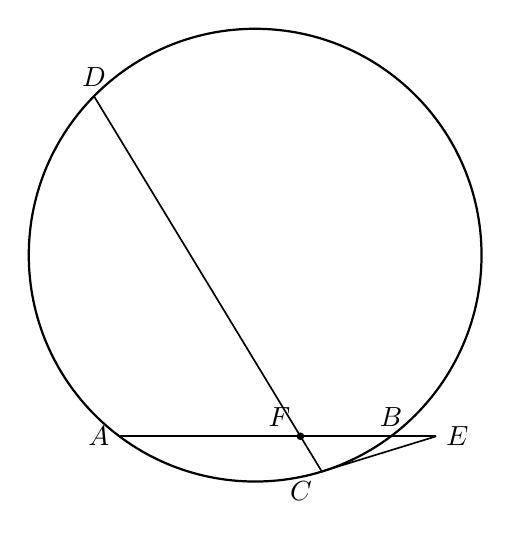
\begin{tikzpicture}[scale=1.15, >=stealth, semithick]
  \coordinate (O) at (-0.5,1);
  \coordinate (A) at (-2,-1);
  \coordinate (B) at (1,-1);
  \coordinate (E) at (1.5,-1);
  \coordinate (F) at (0,-1);
  \coordinate (C) at (0.236,-1.389);
  \coordinate (D) at (-2.28,2.756);

  \draw[thick] (O) circle (2.5);
  \draw (A) -- (E);      % 弦 AB 及其延长线至 E
  \draw (D) -- (C);      % 弦 CD
  \draw (C) -- (E);      % 切线 CE

  \fill (F) circle (1.2pt);

  \node at (A) [left] {$A$};
  \node at (B) [above] {$B$};
  \node at (E) [right] {$E$};
  \node at (F) [above left] {$F$};
  \node at (C) [below left] {$C$};
  \node at (D) [above] {$D$};
\end{tikzpicture}
